\documentclass{article} %article 
\usepackage{graphicx}
\usepackage{amssymb}
\usepackage{xcolor}
\usepackage{listings}
\usepackage{soul}
\usepackage{fancyhdr} 
\usepackage{lastpage}


\pagestyle{fancy} %fancyhdr宏包新增的页面风格
\fancyhf{}
\rhead{Page \thepage\ of \pageref{LastPage}}%当前页 of 总页数
\lhead{\bfseries Team $\# $ 6666666}

\title{Arrangement for DroneGo}  %文章标题
\author{Hao Li, Peisen Wang, Benjia Liu}   %作者的名称
\date{\today}       %日期
% 设置页面的环境,a4纸张大小,左右上下边距信息
\usepackage[a4paper,left=10mm,right=10mm,top=15mm,bottom=15mm]{geometry} 



\begin{document}
\maketitle

\begin{abstract}

% 在波多黎各遭受最严重的飓风袭击后,许多人受伤。高速公路被洪水堵塞并损坏。我们建立了一个模型,可以同时满足药物输送和带有旋翼无人机的道路侦察的需求。
% 我们的模型考虑了以下因素:货运集装箱的数量,无人机的类型和数量,药品的数量,每个货运集装箱的相关包装配置, 货运集装箱的确切位置以及每架无人机的时间表。
After the worst hurricane to ever hit Puerto Rico, lots of people were injured. Highways were blocked and damagedby the flood.
We establish a model to both meet the needs of medicine delivery and road reconnaissance with rotor wing drones.
Our model takes into account the following factors :  the number of cargo containers, the type and the number of drones, 
the number of medicines,  the associated packing configuration of each cargo, the exact locations of cargo containers.

% 第一, 通过对航拍图像进行二值化,形态学膨胀和特征点识别, 将图像转化成一张带有可通行区域(道路)和障碍物区域(非道路区域)的栅格地图并提取ROI(城市)。
% 通过此地图,我们将集装箱放置在靠近沿海且其飞行半径内道路面积最大的地点:分别是(18.10961, -65.81971), (18.43035, -66.03689), (18.45937, -66.74583)
First, by thresholding the aerial image, morphological dilate and feature point recognition, the image is transformed 
into a Occupancy Grid Map with passable area (road) and obstacle area (non-road area) and extract the ROI (city) in the same time.

%首先,我们依据波多黎各各医院间相距的空间距离和对药品的需求量确定了各集装箱的地理分布和对无人机的安排,其中包括了对无人机运输药品和勘察地形两种功能的分类:不能勘察地形但能够承载更多药品的单个F无人机用来运输药品给相距较近的两个医院,其余距离较远的医院选择用4个速度快的无人机B来运输药品。然后余下的45个B型无人机以各个城市为基点对周围的地形进行勘察,既保证了每个医院的药品需求量,又能够极大地提高侦察的有效性。
Second, we determined the geographic distribution of each container and the arrangement of drones based on the spatial distance between Puerto Rico's every hospital and the demand for medicines, which included the classification of two functions of drone , one is transportation Medicine drones, the other is the terrain survey drones: A single F drone that cannot survey the terrain but can carry more medicines is used to transport medicines to two hospitals that are closer to each other,which are located farther away Of hospitals were selected to use 4 fast drones B to transport medicines.Then the remaining 45 B-type UAVs surveyed the surrounding terrain with each city as the base point, which not only ensured the drug demand of each hospital, but also greatly improved the effectiveness of the reconnaissance.

%其次,在进行集装箱装箱的过程中,在利用混合遗传模拟退火算法的前提下,保证药品和无人机都平放在集装箱的底部,使运输过程最大程度的保证稳定性和安全性。在保证了每个医院一个月的药品需求量和充足的勘察无人机数量的前提下,使集装箱容积利用率最优化,最终统计三个集装箱的空间利用率依次为18.08\%、20.56\%、21.68\%。
In the process of container loading, under the premise of using the \textbf{hybrid genetic simulated annealing} algorithm, medicines and drones are placed on the bottom of the container, and stability and safety can be guaranteed to the greatest extent when transporting. On the premise of ensuring a one-month drug demand for each hospital and a sufficient number of survey drones, the container volume utilization rate is optimized, and the space utilization rate of the three containers is 18.08 \%, 20.56 \%, 21.68 \%.

% 第三, 由于每次运输没有过多货物,故简单设计了无人机的有效载荷配置。对于A集装箱:无人机B装载一个MEDIC1。 对于B集装箱:无人机F装载三个MEDIC1,两个MEDIC2, 两个MEDIC3。
% 对于C集装箱:无人机B装载两个MEDIC1或者一个MEDIC3或者一个MEDIC1和一个MEDIC3。
Third, since there are not too many cargo esthest per shipment, the payload configuration of the drone is simply designed. 
For A Containers: Drone B mounts a MEDIC1. For B Containers: Drone F mounts three MEDIC1s, two MEDIC2s, two MEDIC3s.
For C containers: Drone B is loaded with two MEDIC1s or one MEDIC3 or one MEDIC1 and one MEDIC3.

% 第四, 由于栅格地图已经包含了障碍物区域, 所以我们对于城市间的道路信息侦察和交付路线获取采用RRT-connect算法(能够比A* / dijiskra更好地保持在道路的中轴线上)
Fourth, because the Occupancy Grid Map has already contains the obstacle information, we determine to use \textbf{RRT-connect} instead of \textbf{A*} or \textbf{dijiskra} algorithm
to plan the dilvery path and roads between cities.

% 最后, 我们得到的结果是可以维持一个月的药物运输,在飞行半径内的道路侦察覆盖率为100%, 对于连接偏远城市的道路侦察为100%
At last, the result we got is we can sustain a month of medicine supply, 100\% road reconnaissance coverage within the flight radius
and 100\% road reconnaissance between cities.
\end{abstract}

\tableofcontents

\section{Introduction}                             %——一号子标题  China is in East Asia.
     \subsection{Background}                      %——二号子标题  Beijing is the capital of China                 
         \paragraph{}In 2017, the island's worst hurricane hit the territory of Puerto Rico in history, which killed more than 2,900 people ,causing severe damage to the island. The violent storm destroyed most of the island's cellular communications and power services systems. What’s worse, flooding blocked and damaged many of the island's highways and roads, leaving the extent of damage to various parts of the island of Puerto Rico unclear.


As time goes by, the rescue and treatment of the people on the island is imminent! Due to the huge increase in the use of medical supplies and the urgent need for rescue organizations to understand the road conditions in various places,we need to design a portable disaster response system called "DroneGo" to assist rescue and assist HELP Inc. improve it response capabilities.
We will make full use of the drones to transport the medical supplies needed, while providing high-resolution videos of the damaged and repairable transportation road network through the drones, which are able to prepare for the rescue and further reconstruction of the disaster area.

       \subsection{Restatement}
         \paragraph{}Considering the requirements and conditions given in the background information and questions, we will complete the following questions:


\textbf{(1)} For the HELP Inc. DroneGo disaster response system, a drone fleet configuration system and a medical kit configuration system are recommended. These systems need to meet the requirements of the Puerto Rico Hurricane Program

\textbf{(2)} Design relevant packaging configurations for each of up to three ISO cargo containers to transport the system to Puerto Rico.


\textbf{(3)} Determine the optimal location for placing containers of the DroneGo disaster response system on Puerto Rico Island (the number of containers in each location is less than or equal to 3) in order to provide material preparation for medical supply and video surveillance of the road network.

\textbf{(4)} Provide payload packaging configurations ( medical packaging in the drone's cargo bay), delivery routes and schedules for each drone included in the DroneGo fleet to meet the emergency medical care identified in the Puerto Rico Hurricane scenario Packaging requirements.


\textbf{(5)} Provide a drone flight plan that enables the DroneGo fleet to use car cameras to evaluate major highways and roads to support HelpInc's mission.

\section{Assumptions and Justifications}  
 \paragraph{}We make some general assumptions to simplify our model. These assumptions and corresponding reasons are listed below:

\textbf{(1)} For simplicity, we made this assumption as follows. The weight of the cargo will not affect the maximum range of the drone used. That is to say, no matter whether there is cargo or not, the drone’s maximum sailing distance is exactly the same. In fact, the weight of delivered drones is often greater than the weight of their cargo. It is reasonable to ignore the effect of cargo weight. This will greatly simplify our model.

\textbf{(2)} Helicopters can transport containers to any designated location we have established in the disaster area. In the affected areas, timely external assistance is urgently needed to restore order. Therefore, we consider air transport rather than sea transport. Although Puerto Rico is an island, air transport will bring adaptability to our model in other cases.

\textbf{(3)} We have a plan for transportation in most normal cases, so we can ignore the influence of factors such as harsh environment and extreme weather when the drones fly.


\textbf{(4)} The drones can be recycled, and it can be charged by returning to the starting place for the next use. Because drones are more than expensive and DroneGo is an NGO . As a result, we should focus on financial costs.


\textbf{(5)} When using containers to transport drones and medical packaging, the transportation time is long, the quantity of goods is large, and the weight is heavy. Therefore, we have added a buffer to the container, and we believe that medical packaging can only be placed in the container on the front side, not upright or inverted. Of course, medical packaging can be rotated horizontally to increase space utilization when placing containers. When transporting medical packaging by drones, the transportation time is shorter, the number of goods is smaller, and the weight is lighter, so we believe that medical packaging can be placed in the drone cargo compartment in various ways.


\textbf{(6)} Assume that drone communication and data transfer are always available. We can achieve telephone communication through radio communication or satellite communication. Drone communication does not rely on ground equipment.

\section{Notations}

\section{Model Establishment}
\paragraph{}Before building the model, we first address the following issues.
First of all, when designing the number of drones and medical kits, delivery routes and other tasks, the most basic goal must be to enable the drones to meet the daily needs of the hospital. What’s more, while satisfying the needs, it should investigate the main traffic routes as much as possible, and obtain road video information in time to prepare for daily rescue.
Last, considering the high cost of drones, we want to reduce the number of drones as much as possible so that ISO containers can have more space for more medical packages.
In short, we will choose as few drones as possible to meet the most basic needs of each hospital, and use the selected drones to perform the maximum video surveillance in the affected area.
\subsection{ROI Extract And Map Established}

\subsubsection{The ratio of the image between the real world}

    Through calculation we can got the ratio $R$ of the physical distance corresponding to each pixel. 
    This is of great significance for our future flight radius calculation and path planning. We extract
    two points $A$($x_A$, $y_A$) and $B$($x_B$, $y_B$) in the image,  calculate euclidean distance between $A$ and $B$
    (unit : $pixel$), measure their physical distance $S_{real}$ using Google Map.
    
\centerline{$R=\frac{S_{real}}{\sqrt{\left(x_{A}-x_{B}\right)^{2}+\left(y_{A}-y_{B}\right)^{2}}} = \frac{69.61 km}{615.11 pixels} = 113.1 m/pixel$}

\subsubsection{Threshold The Image} 
    Load the original image and convert it into the threshold image so we can extract the road data from the orignal image.
    It makes us possible to reconnaissance along the road.The range is from$(50,  50, 20)$ to $(150,  90, 50)$

    \lstset {language=C++}
        \begin{lstlisting}
            cv::Scalar lower_range = { 50,  50, 20 };
            cv::Scalar upper_range = { 150,  90, 50 };	
            cv::inRange(src, lower_range, upper_range, out);
    \end{lstlisting}

    \begin{figure}[h]
        \centering
            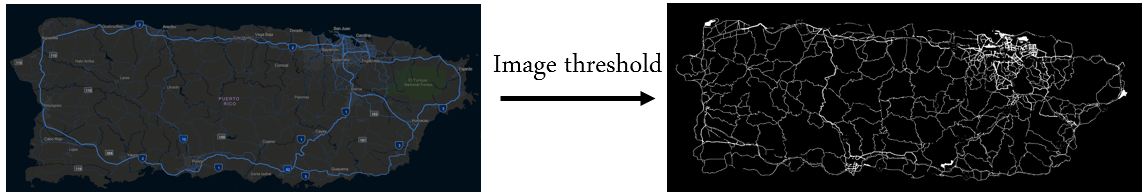
\includegraphics[scale=0.6]{threshold.png}
        \caption{Shows the result after threshold.}
    \end{figure}
\subsubsection{Dilated The Image} 
    We dialte the image (using $8 * 8$ Convolution kernel).On the one hand, the new white area represents the area that our drone can detect, on the other hand, 
    this can be our better plan for the reconnaissance trajectory and delivery route of the medicine.
    
    \centerline{Convolution Kernel $=\left[\begin{array}{cccccccc}{1} & {1} & {1} & {1} & {1} & {1} & {1} & {1} \\ {1} & {1} & {1} & {1} & {1} & {1} & {1} & {1} \\ {1} & {1} & {1} & {1} & {1} & {1} & {1} & {1} \\ {1} & {1} & {1} & {1} & {1} & {1} & {1} & {1} \\ {1} & {1} & {1} & {1} & {1} & {1} & {1} & {1} \\ {1} & {1} & {1} & {1} & {1} & {1} & {1} & {1} \\ {1} & {1} & {1} & {1} & {1} & {1} & {1} & {1} \\ {1} & {1} & {1} & {1} & {1} & {1} & {1} & {1} \\ {1} & {1} & {1} & {1} & {1} & {1} & {1} & {1}\end{array}\right]$}

    \lstset {language=C++}
        \begin{lstlisting}
            cv::Mat element = cv::getStructuringElement(cv::MORPH_RECT, cv::Size(8, 8));
            cv::dilate(out, out_dilated, element);
    \end{lstlisting}

    
    \begin{figure}[h]
        \centering
            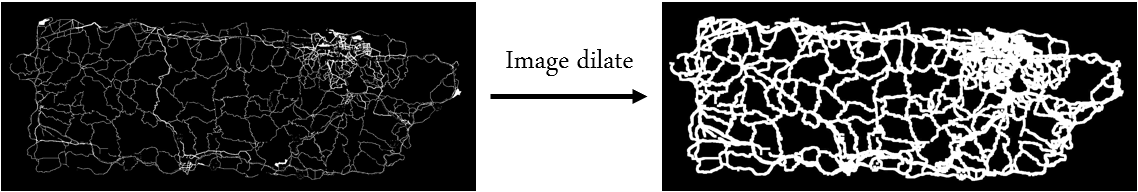
\includegraphics[scale=0.6]{dilate.png}
        \caption{Shows the result after dilated.}
    \end{figure}

\subsubsection{Detct And Extract The Cities Location}
By performing image feature detection and circle fitting, 
we can extract the locations of various cities for later road reconnaissance.
    \lstset {language=C++}
    \begin{lstlisting}
        medianBlur(src, cimg, 5);
        GaussianBlur(cimg, cimg, Size(9, 9), 2, 2);
        Canny(cimg, cimg, 10, 250, 5);
        vector<vector<Point>>cnts;
        findContours(cimg, cnts, RETR_EXTERNAL, CHAIN_APPROX_NONE);
        for (int i = 0; i < cnts.size(); i++)
        {
            vector<Point> cnts_single = cnts[i];
            if (cnts_single.size() > 0)
            {
                vector<Point> approx;
                string shape = detect(cnts_single, approx);
                Moments M = moments(cnts_single);
                int cX, cY;
                if (M.m10 != 0)
                {
                    cX = int((M.m10 / M.m00));
                    cY = int((M.m01 / M.m00));
                }
                putText(cimg, IntToStr(cX) + " , " + IntToStr(cY), Point(cX, cY),
                 FONT_HERSHEY_SIMPLEX, 0.5, Scalar(255, 0, 255), 1);  
            }
        }
    \end{lstlisting}

    \begin{figure}[h]
        \centering
            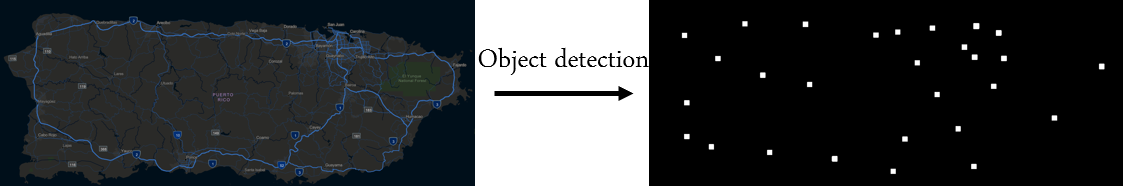
\includegraphics[scale=0.6]{object_detection.png}
        \caption{Shows the result after object detection.}
    \end{figure}

    \subsection{Related analysis of hospitals and drones}
\subsubsection{Analysis of hospital location and material needs}
\paragraph{}To recommend drone fleets and medical kits to HELP, we should understand the basics of the Puerto Rican disaster firstly. The locations of the five hospitals given in the question are shown in Figure 1. We will analyze the demands of these hospitals and make drone selection based on the location of the hospitals.
\begin{figure}[htb] 
 \center{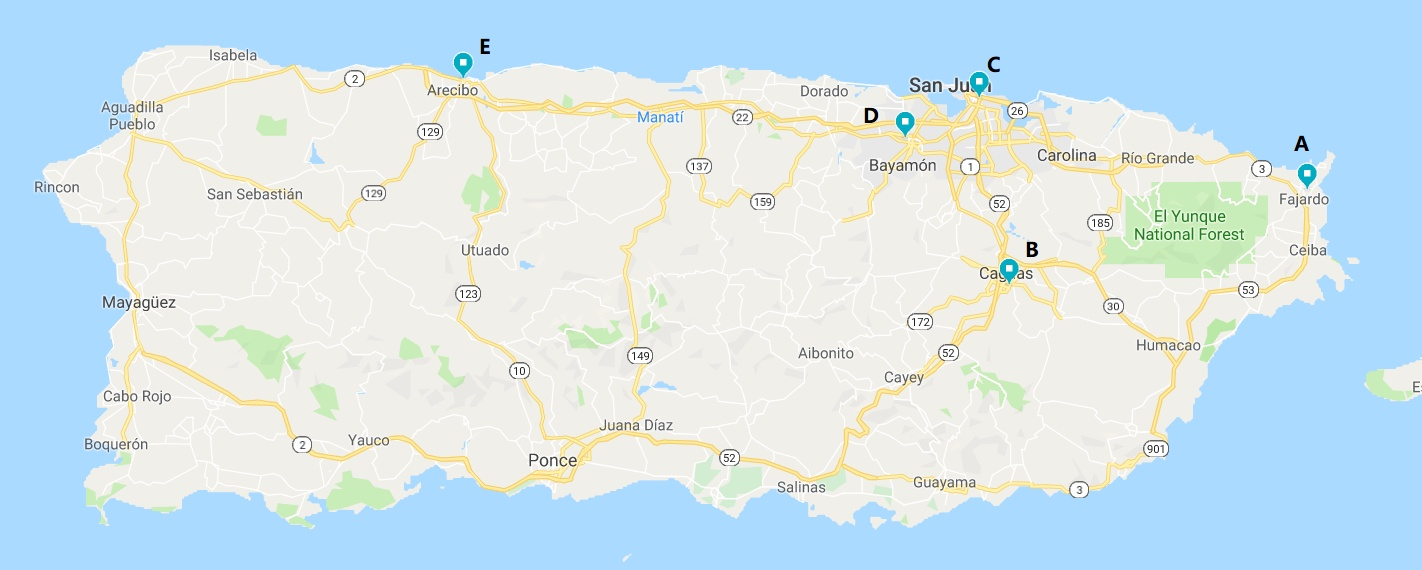
\includegraphics[width=10cm]  {3.jpg}} 
 \caption{\label{1}Map of Puerto Rico} 
 \end{figure}
\paragraph{}Based on the idea of minimizing the number of drones.For two hospitals with distance $S\left(h_{m}, h_{n}\right)$, $h_{n}$ and $h_{m}$.The weights of the medical packages they need are $M p_{m}$and$M p_{n}$.As long as any drones can be found, its maximum flight distance$D_{i}$and payload$Z_{i}$ meet the requirements:

\centerline{$\left\{\begin{array}{l}{S\left(h_{m}, h_{n}\right) \leq D_{i}} \\ {M p_{m} \leq Z_{i}} \\ {M p_{n} \leq Z_{i}}\end{array}\right.$                             \qquad  \qquad  \qquad       (1)}

\paragraph{}It is possible to use the same drone to distribute medicines to multiple hospitals.Next, we started to pay attention to the needs of the hospital every day. We integrated the medical packages required by each hospital every day, as shown in the following chart 2:


\centerline{\textbf {Demand for medical kits}}
\begin{table}[h]
\begin{tabular}{cccc}
\hline
\textbf{HospitalName} & \textbf{MED1} & \textbf{MED2} & \textbf{MED3} \\ \hline
Caribbean Medical Center Jajardo         & 1         & 0       & 1        \\
Hospital HIMA San Pablo            & 2         & 0        & 1        \\
Hospital Pavia Santurce San Juan         & 1         & 1              &0                   \\ 
Puerto Rico Children's Hospital Bayamon         & 2         & 1              &2                  \\ 
Hospital Pavia Arecibo Arecibo        & 1         & 0             &0                   \\ 
SUM         & 7       & 2              &4                  \\ 
\hline
\end{tabular}
\end{table}
\subsubsection{Comparison of drones}  
\paragraph{}We uphold the concept of economy and use as few drones as possible while satisfying the basic material delivery conditions.Therefore, we compared the load capacity, the volume and the running distance of the drone from the table, and selected two types of drones, B and F.We can conclude that although the drone B has a small payload, it has the longest flight distance and a small volume, so it is very suitable for the supply of medical supplies to Pavia Arecibo Hospital.For UAV F, it has the largest load capacity and a very long flight distance, which is very suitable for the medical supplies of the other four hospitals.

From the question we can know the basic information of the drones as follows:


\centerline{\textbf {Basic information about drones}}
\begin{table}[h]
\begin{tabular}{cccc}
\hline
\textbf{Type of drone} & \textbf{Load capacity/lbs} & \textbf{Total flight distance/km} & \textbf{volume/cuft} \\ \hline
A         &          3.5& 23.33       & 50625        \\  \hline
B            &         8 & 52.67        & 19800        \\  \hline
C         &          14& 37.33              &90000                   \\   \hline
D         & 11        & 18              & 12500                 \\   \hline
E       &          15& 15            &    13500               \\ \hline
F         &       22 & 31.6              &  40000                \\ \hline
G         &       20&   17.07            &     17408             \\  
\hline
\end{tabular}
\end{table}  
\subsubsection{selection of drones} 
\paragraph{}Based on the above analysis of the needs of the hospital, the analysis of the location of the hospital, and the analysis of the choice of drones, we choose:
A type B drone transported medical supplies to Pavia Arecibo Hospital;An F-type drone supplies medical supplies to Hospital Pavia Santurce San Juan and Puerto Rico Children's Hospital Bayamon;A Type B drone carries medical supplies to the Caribbean Medical Center Jajardo;Two Type B drones transported medical supplies to Hospital HIMA San Pablo, one of which transported a medicine number three and the other transported two medicine number one.After solving the supply of medical supplies, we are now considering the issue of drone allocation for road reconnaissance.
In this question, we selected drones by assigning criteria to large, medium and small cities near five hospitals.
The distribution of cities near the five hospitals is shown below:


\begin{figure}[htb] 
 \center{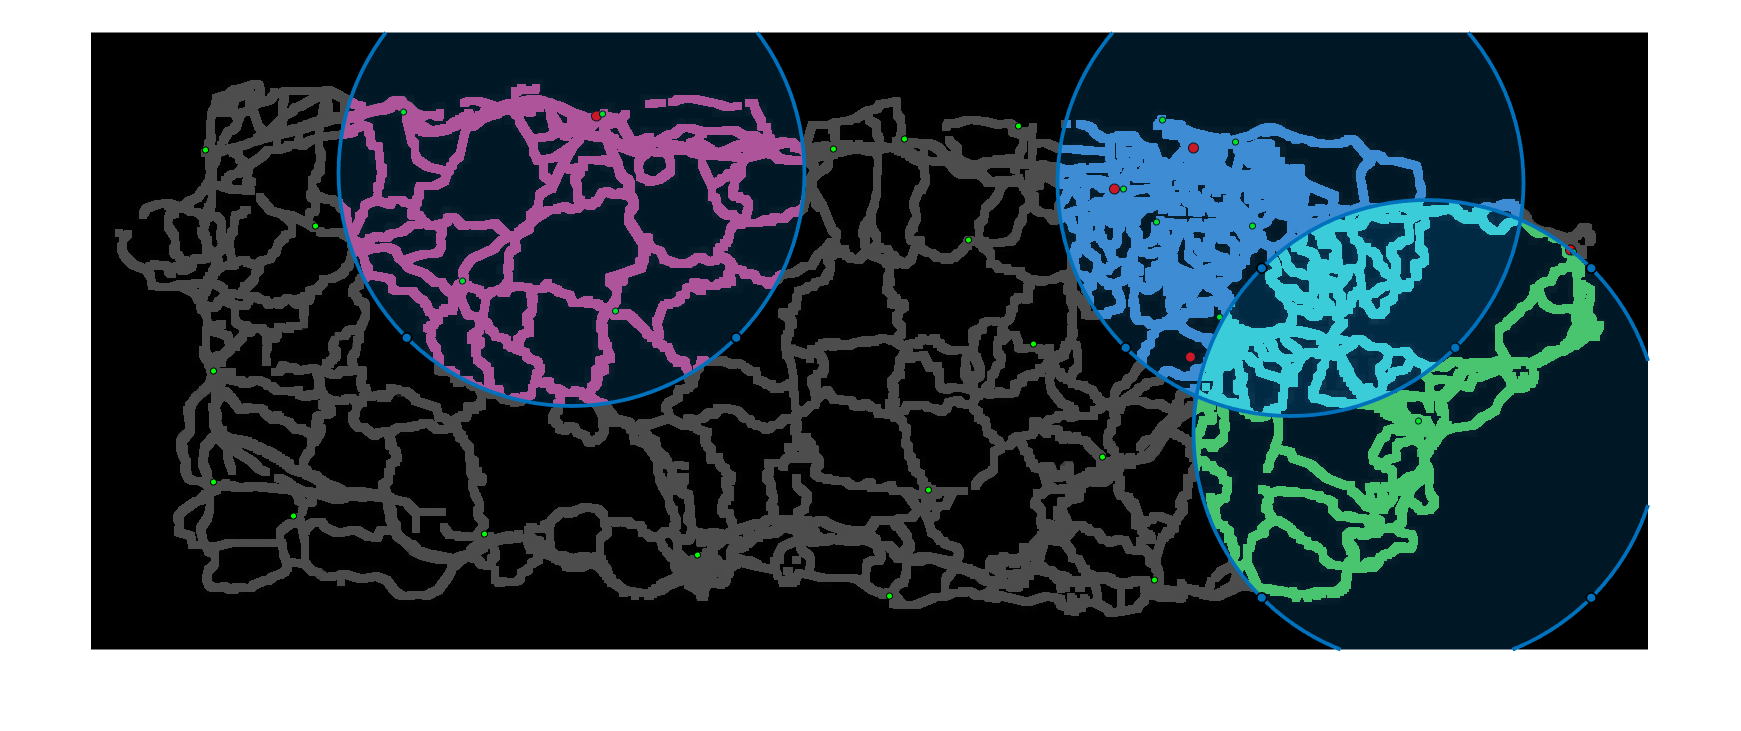
\includegraphics[width=10cm]{2.png}} 
 \caption{\label{1}Map of main city} 
 \end{figure}
We chose the larger one as the main reconnaissance destination, as shown by the green dot in the figure above.


We will prepare 11 Type B drones near Pavia Arecibo Hospital, and select 14 Type B UAVs near the other four hospitals for road reconnaissance.
\subsection{Container packing design}
Since we have given the basic scheme of drone selection and the basic information of demand and supply of the five hospitals above, in this part, we will carry out the optimization of the container packing problem. These include a three-container joint design of drones and medical supplies.
\subsubsection{Problem Description} 
\paragraph{}The container loading problem is defined as:Given i containers with length,width and height of L $ _i $, W $ _i $, H $ _i $ and j types of length, width and height of l $ _j $, w $ _j $, h $ _j $ , Goods with a weight of m $ _j $.While considering certain constraints, and on the premise of meeting the supply of medicines, transport drones and medicine boxes as safely as possible.


Restrictions:

         \textbf{(1)} Volume constraints: During the loading of containers, space is continually shrinking, and container volume and cargo volume are the main criteria for loading feasibility.

         \textbf{(2)} Orientation constraint: When determining the loading order of goods, it is also necessary to consider the impact of loading in different directions on space utilization. Ensure that drugs and drones remain stable during transportation.

         \textbf{(3)} Loading order constraints: Different drones and medicines should be loaded according to different loading order priorities.
\subsubsection{Model assumptions} 
The algorithm mainly studies the container loading layout. In order to improve the space utilization of the container, the maximum utilization of the container volume is used as the objective function.
The following assumptions are made in the model:

\textbf{(1)} There are no regional restrictions on the location inside the container

\textbf{(2)} Good quality distribution

\textbf{(4)} The goods can maintain their shape and size without being deformed by stacking.

\subsubsection{Model building} 
Based on the above content analysis, the objective function and packing constraints of the current mathematical model are established as follows:


\textbf{(1)}Objective function is optimal for container volume utilization


\centerline{$Z=\max \frac{\sum_{i=1}^{n} v_{i}}{V}$}
Among them, Z is the volume utilization rate of the container, i is the serial number of the cargo, i = 1, 2, ..., n. v $ _i $ is the volume of the i-th cargo, and V is the volume of the container.

\textbf{(2)}Cargo total volume constraint

\centerline{$\sum_{i=1}^{n} v_{i} \leqslant V$}

\textbf{(3)}3D dimensional constraints for cargo loading

\centerline{$\left\{\begin{array}{l}{0 \leqslant x_{i}+l_{i} \leqslant L} \\ {0 \leqslant y_{i}+w_{i} \leqslant W} \\ {0 \leqslant z_{i}+h_{i} \leqslant H}\end{array}\right.$}

Among them, x $ _i $, y $ _i $, z $ _i $ are the reference coordinates of the goods placement position, l $ _i $, w $ _i $, h $ _i $ are the length, width, and height of the goods, L, W, H For the length, width, and height of the container.
\subsubsection{Solving Algorithm}
\textbf{(1)}Three-space segmentation heuristic


The three-dimensional boxing problem itself has certain complexity, and an efficient loading scheme is generated by using a three-space segmentation heuristic algorithm.
The heuristic algorithm can generate high-quality solutions in a short time, and also has the flexibility to adapt to different needs. Here are the rules of the heuristic algorithm.

    \textbf{(A)}: Ordering rules

The order of cargo loading will affect the quality of the container space layout. In the process of designing the loading scheme, in order to determine the order in which the goods are placed in the container, sequencing rules are more commonly used.

This time is the commonly used rule of decreasing longest edge.
First compare the longest side of the cargo, if the longest side is the same, compare the second longest side, and then load along the length of the container;
If the longest side and the second longest side of the goods are the same, then consider the volume of the goods and fill them in descending order.

Therefore, during the packing process, the drone is first loaded, and then the medicine can be loaded.

    \textbf{(B)}: Positioning rules

In the process of packing the goods to be loaded one by one in a certain sequence, corresponding positioning rules are required to determine their placement.
First place the cargo at one corner of the container, then load them along the sides one by one, and then fill the corners.

   \textbf{(C)}: Space segmentation rules

The remaining space of the container refers to the remaining space in the container that can be used after the cargo is loaded.
In the subsequent process of continuously adding goods, the shape of the remaining space has become relatively complicated, and it is difficult to describe it overall.
In order to make the cargo space to be expressed clear, the three-space division rule is used to divide the container space.When a container is loaded with a cargo, the space structure in the container changes at this time. Except for the volume occupied by the cargo, the remaining space is divided into the front, right, and upper parts.When the goods are continuously added, the above-mentioned subspaces are successively generated until the container is filled or there is no cargo to be held.


The following figure is the corresponding relationship between the container's three-space partition layout and the three-dimensional coordinate system:
\begin{figure}[h]
    \centering
    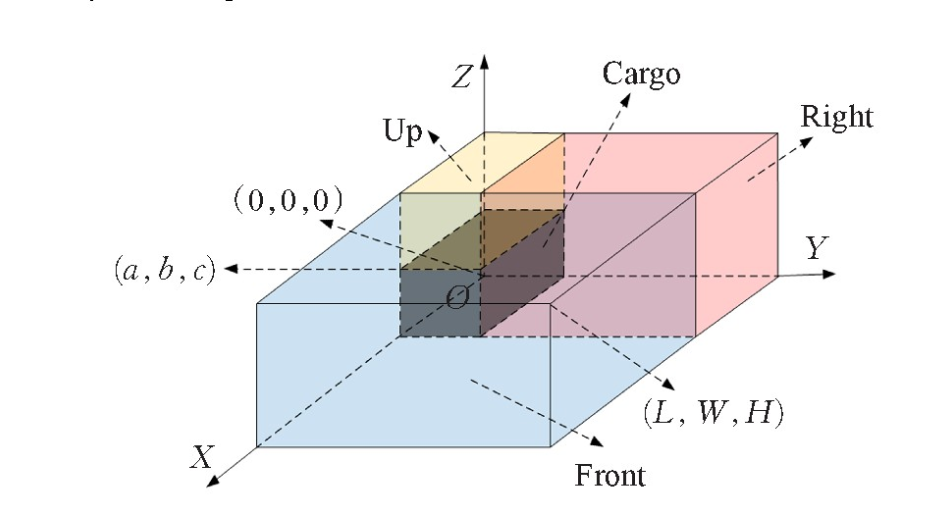
\includegraphics[scale=0.6]{99.png}
    \caption{Division of remaining space}
\end{figure}
The specific encoding of the heuristic algorithm is as follows:

\centerline{$V=\left(i, x_{a}, y_{a}, z_{a}, x_{b}, y_{b}, z_{b}\right)$}
In the above coding sequence, i represents the serial number of the container, X $ _a $, Y $ _a $, and Z $ _a $ represent the three-dimensional coordinates of the reference point that can be placed in this space, that is, the coordinates of the lower left and lower vertices of the space.
When the three-dimensional coordinates where the reference point can be placed are the origin, the length, width, and height of the space are X $ _b $, Y $ _b $, Z $ _b $;
When the three-dimensional coordinates of the placeable reference point are not the origin, the length of the space is expressed as:
\centerline{$L=\max \left(x_{b}-x_{a}, y_{b}-y_{a}\right)$}
The width is expressed as:

\centerline{$W=\min \left(x_{b}-x_{a}, y_{b}-y_{a}\right)$}

The height is expressed as:

\centerline{$H=z_{b}-z_{a}$}

It can be known from the above coding rules that if the length of the container is L, the width is W, and the height is H, then the initial available space of the container is expressed as

\centerline{$V=(i, 0,0,0, L, W, H)$}
For example, after a piece of cargo with length a, width b, and height c is loaded into the container according to the method shown in Figure 1, the code and size of the newly generated three remaining spaces V (m) are:

\centerline{$\left\{\begin{array}{l}{V(m)=(i, a, 0,0, L, W, H)} \\ {L_{m}=\max (L-a, W)} \\ {W_{m}=\min (L-a, W)} \\ {H_{m}=H}\end{array}\right.$}

The encoding size of V (m + 1) is:

\centerline{$\left\{\begin{array}{l}{V(m+1)=(i, 0, b, 0, a, W, H)} \\ {L_{m+1}=\max (a, W-b)} \\ {W_{m+1}=\min (a, W-b)} \\ {H_{m+1}=H}\end{array}\right.$}

The encoding and size of V (m + 2) is

\centerline{$\left\{\begin{array}{l}{V(m+2)=(i, 0,0, c, a, b, H)} \\ {L_{m+2}=\max (a, b)} \\ {W_{m+2}=\min (a, b)} \\ {H_{m+2}=H-c}\end{array}\right.$}


     The division of the remaining space of the container is a prerequisite for the continued loading of the cargo. Before the container is fully loaded, the remaining space will be continuously generated, so the available remaining space must be searched out.
In the process of searching for the remaining space, the height of the space is sorted in ascending order, and the priority of the space to be loaded is specified, thereby ensuring that the goods are loaded from bottom to top.
\textbf{(2)}Space merging rules
The space segmentation of the heuristic algorithm finds the available remaining space for the loading of the cargo.
However, in the process of actually writing the algorithm, there will be some scattered space that cannot be used, so it must be integrated in a certain way.
Space merger is to make full use of the scattered space to form a larger space to be installed.
This will not only improve the space utilization of the container, but also improve the loading effect of the cargo.
Define K (l) = (X $ _i $, Y $ _i $, Z $ _i $, X $ _j $, Y $ _j $, Z $ _j $), l is the random space sequence number of the set K (l), The length of the idle remaining space fragments is:

\centerline{$L_{l}=\max \left(x_{j}-x_{i}, y_{j}-y_{i}\right)$}
The width is expressed as:

\centerline{$W_{l}=\min \left(x_{j}-x_{i}, y_{j}-y_{i}\right)$}

The height is expressed as:

\centerline{$I I_{l}=z_{j}-z_{i}$}

In the process of designing the algorithm, the container is placed in a three-dimensional coordinate system, so spatial merging includes merging in three directions.

\textbf{(3)}{Three-space segmentation heuristic algorithm steps}

According to the design concept of the three-space segmentation heuristic algorithm, combining the ordering rules, positioning rules, space segmentation rules, and space merger rules, the ordering and control of the cargo loading process is made.

Step 1: Import the basic data of the container, the drone, and the medicine, define the number of cargo types, the total number of cargoes, and the container serial number through function variables, and initialize the remaining space of the container according to the space coding rules.

\begin{table}[htp]
\begin{tabular}{|c|c|c|c|c|c|c|c|c|}
\hline
\multicolumn{9}{|c|}{\begin{tabular}[c]{@{}c@{}}Table 1. Standard ISO\\ Container Dimensions\end{tabular}}                                                                                                                                                                                                                                                                                                                                                                                                                            \\ \hline
& \multicolumn{3}{c|}{Exterior}                                                                                                                                           & \multicolumn{3}{c|}{Interior}                                                                                                                                           & \multicolumn{2}{c|}{Door opening}                                                                              \\ \hline
                                                                           & \begin{tabular}[c]{@{}c@{}}Length\\ (in.)\end{tabular} & \begin{tabular}[c]{@{}c@{}}Width\\ (in.)\end{tabular} & \begin{tabular}[c]{@{}c@{}}Height\\ (in.)\end{tabular} & \begin{tabular}[c]{@{}c@{}}Length\\ (in.)\end{tabular} & \begin{tabular}[c]{@{}c@{}}Width\\ (in.)\end{tabular} & \begin{tabular}[c]{@{}c@{}}Height\\ (in.)\end{tabular} & \begin{tabular}[c]{@{}c@{}}Width\\ (in.)\end{tabular} & \begin{tabular}[c]{@{}c@{}}Height\\ (in.)\end{tabular} \\ \hline
\begin{tabular}[c]{@{}c@{}}20’\\ Standard \\ Dry\\  Container\end{tabular} & 240                                                    & 96                                                    & 102                                                    & 231                                                    & 92                                                    & 94                                                     & 2                                                     & 89                                                     \\ \hline
\end{tabular}
\end{table}
\begin{table}[htp]
    \begin{tabular}{|c|c|c|c|c|c|c|c|}
    \hline
          & \multicolumn{3}{c|}{\begin{tabular}[c]{@{}c@{}}Shipping\\ Container\\ Dimension\end{tabular}}                                                                           &                                                                            & \multicolumn{3}{c|}{\begin{tabular}[c]{@{}c@{}}Configuration\\ Capabilities\end{tabular}}                                                                                               \\ \hline
    Drone & \begin{tabular}[c]{@{}c@{}}Length\\ (in.)\end{tabular} & \begin{tabular}[c]{@{}c@{}}Width\\ (in.)\end{tabular} & \begin{tabular}[c]{@{}c@{}}Height\\ (in.)\end{tabular} & \begin{tabular}[c]{@{}c@{}}Max Payload\\  Capability\\ (lbs.)\end{tabular} & \begin{tabular}[c]{@{}c@{}}Video\\ Capable\end{tabular} & \begin{tabular}[c]{@{}c@{}}Medical\\ package\end{tabular} & \begin{tabular}[c]{@{}c@{}}Drone\\ Cargo\\ Bay Type*\end{tabular} \\ \hline
    B     & 30                                                     & 30                                                    & 22                                                     & 8                                                                          & Y                                                       & Y                                                         & 1                                                                 \\ \hline
    F     & 40                                                     & 40                                                    & 25                                                     & N                                                                          & Y                                                       & Y                                                         & 2                                                                 \\ \hline
    \end{tabular}
    \end{table}

\begin{table}[htp]
    \begin{tabular}{|c|c|c|l|l|}
    \hline
Drone Cargo Bay Type & Length(in.) & Width(in.) & Height(in.) &            \\ \hline
    1                    & 8           & 10         & 14          & Top Loaded \\ \hline
    2                    & 24          & 20         & 20          & Top Loaded \\ \hline
    \end{tabular}
    \end{table}
\begin{center}
    \begin{table}[htp]
        \begin{tabular}{|c|c|c|}
        \hline
\multicolumn{3}{|c|}{Emergency Medical Package Configuration} \\ \hline
        Package ID  & Weight (lbs.) & Package Dimension (L*W*H   in.)  \\ \hline
        MED 1       & 2             & 14*7*5                          \\ \hline
        MED 2       & 2             & 5*8*5                           \\ \hline
        MED 3       & 3             & 12*7*4                          \\ \hline
        \end{tabular}
    \end{table}
    \end{center}
Step 2: Code the placement of the goods:

\centerline{C=(i,j,x,y,z,l,w,h)}

Among them, i is the container number of the container, j is the type number of the cargo, x, y, and z are the starting coordinate points of the cargo, and l, w, and h are the length, width, and height of the cargo.

Step 3: Determine the size of the cargo to be placed in the container and the maximum volume of the container. The length, width, and height of the cargo are less than the length, width, and height of the remaining space in the container.

Step 4: When the cargo meets the above loading requirements, it will be loaded according to the above coding method. After loading, three subspaces are generated according to the space partitioning rules, namely the front space, the right space, and the upper space. Each time the remaining space set is generated, the space is merged according to the space merge rules.

Step 5: Sort the Z coordinates in the remaining space, and then determine the height of the space to ensure that the goods are loaded from bottom to top.

Step 6: Return to step 3, and load subsequent goods in turn until the goods sequence set is empty.

Step 7: When the remaining space of the container cannot satisfy the cargo loading, it is necessary to restart the packing.

Step 8: Finally, the data of loading result and remaining space are obtained. [1]

\subsection{Drone flight path selection}
After solving the problem of packing medical packages and drones, we began to plan the placement of containers and the drone flight routes.
We found a road along the coastline in Puerto Rico's highway network, and we decided to choose three locations on the coast as containers for the containers.
\subsubsection{Selection of container placement location}


\begin{figure}[h]
    \centering
    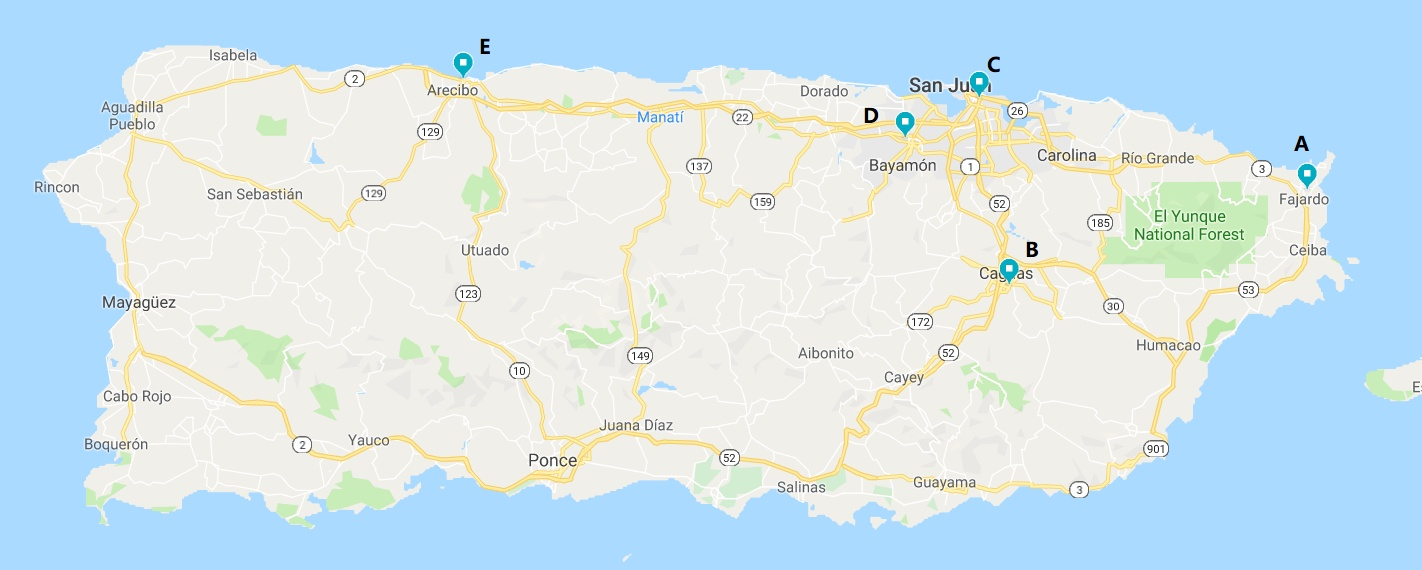
\includegraphics[scale=0.2]{3.jpg}
    \caption{Location of the hospital}
\end{figure}


\textbf{For the medical point above D  B and C:}


\textbf{(1)} Use the RRT algorithm to obtain the path curve at the upper and lower ends of the right-hand ring road from [120, 711] to [151, 1200].


\textbf{(2)}Extracting sample points on a path curve.


\begin{figure}[h]
    \centering
    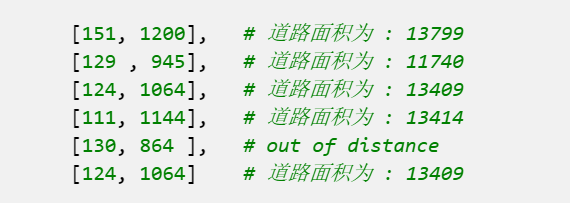
\includegraphics[scale=0.7]{61.png}
    \caption{Location of the CITY}
\end{figure}


\textbf{(3)}Loop through all points and draw circles.


\textbf{(4)}Traverse the area of the road and select the point with the largest value. Use an unexpanded binary map .(you don't need to check whether the torus contains medical centers that should be included because it must be included)


\textbf{(5)}Get [130, 864], road area is: 103851 area is the largest.


\textbf{For the medical point on the left E:}


\textbf{(1)}Use the RRT algorithm to obtain the path curve from [86, 233] to [107, 545] on the right and left ends of the roundabout road


\textbf{(2)}Extract sample points on the path curve


\begin{figure}[h]
    \centering
    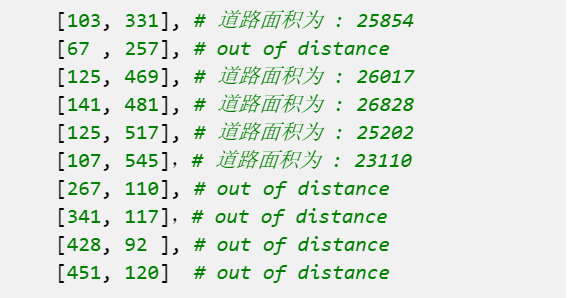
\includegraphics[scale=0.7]{62.png}
    \caption{Location of the CITY}
\end{figure}


\textbf{(3)}Iterate through all points and draw circles


\textbf{(4)}(It is not necessary to check whether the medical center should be included in the torus, because it must be included.) Traverse the road area and select the point with the largest value. Use an unexpanded binary map.


\textbf{(5)} Get point [141, 481], road area is: 54368 area is the largest

\textbf{For the medical point on the right A:}


\textbf{(1)}Use the RRT algorithm to obtain the path curve on the right and left ends of the roundabout road from [455, 1314] to [266, 1498].


\textbf{(2)}Extracting sample points on a path curve.


\begin{figure}[h]
    \centering
    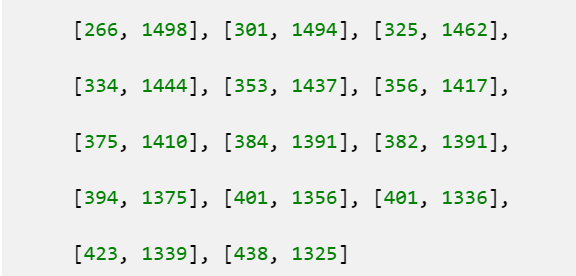
\includegraphics[scale=0.7]{63.png}
    \caption{Location of the CITY}
\end{figure}


\textbf{(3)}Loop through all points and draw circles.


\textbf{(4)}See if the circle contains medical centers that should be included, and if so, traverse the road area and select the point with the largest value.


\textbf{Drawing with matlab}


\textbf{(1)}Combine left, top,and right ROIs into img highlight in the form of imadd ().


\textbf{(2)}Add img highlight and img at a$$3: 7$$ratio to get res img.


\begin{figure}[h]
    \centering
    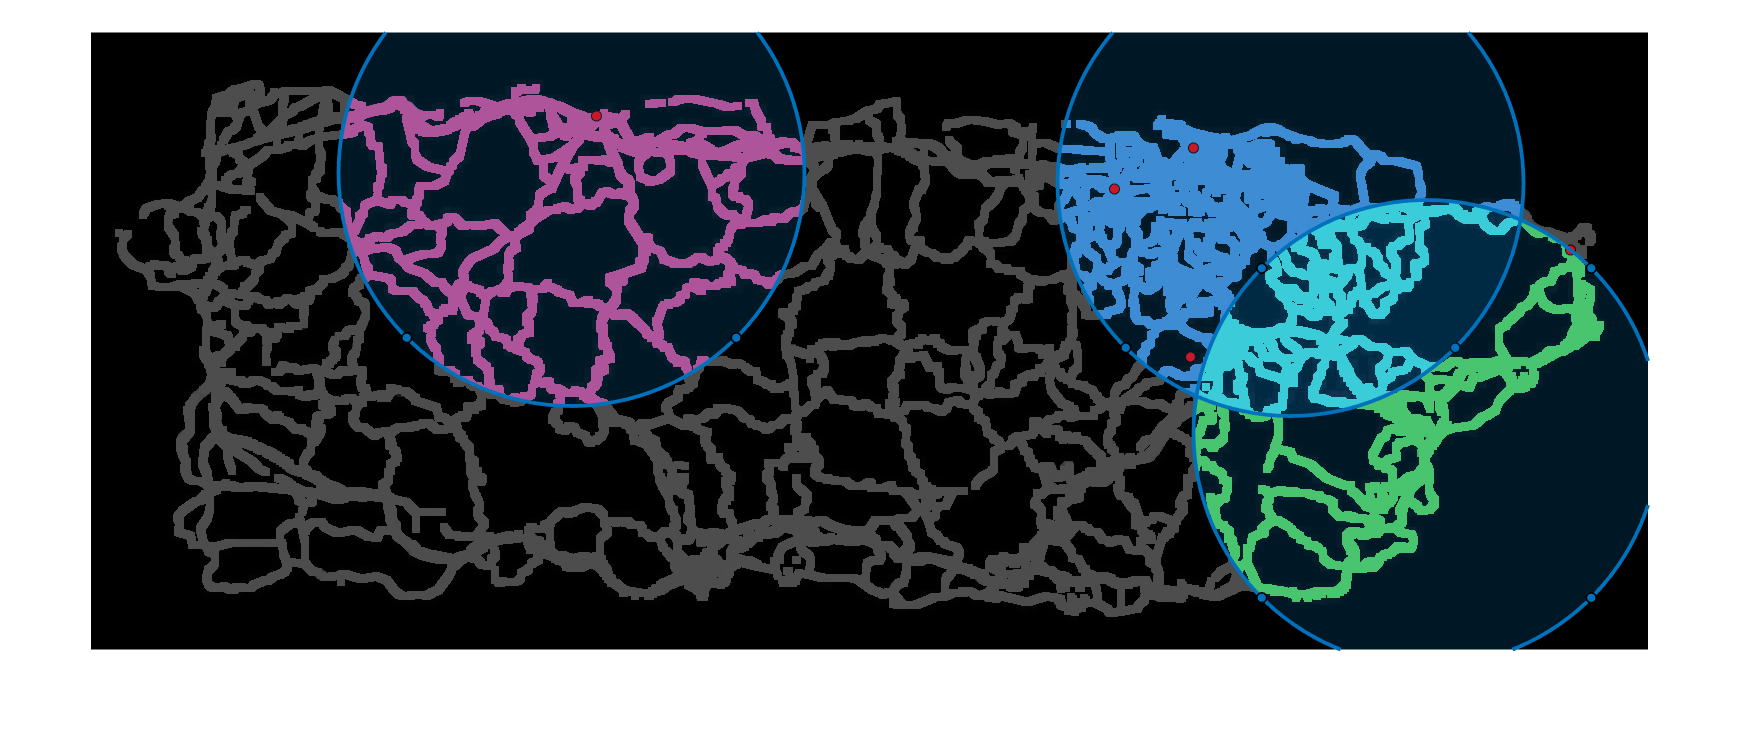
\includegraphics[scale=0.3]{64.png}
    \caption{Location of the CIRCLE}
\end{figure}


\textbf{OpenCV detection city}


\textbf{(1)}Using OpenCV (C ++) to detect urban features.


\textbf{(2)}Get the center pixel coordinates of a city.


\begin{figure}[h]
    \centering
    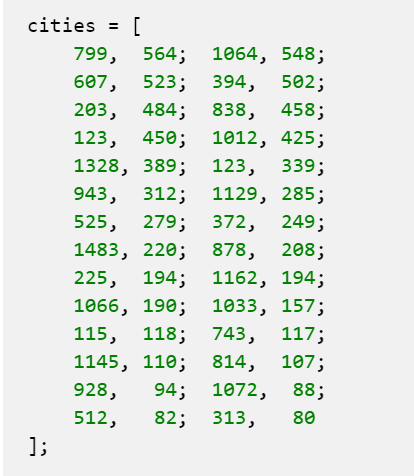
\includegraphics[scale=0.7]{65.png}
    \caption{ the City coordinates}
\end{figure}


\textbf{(3)}List city coordinates as the main reconnaissance destination.


\textbf{Find the Euclidean distance between each city and the landing point using MatLab}


City points assigned to left.
City points assigned to right.
City points assigned to up.


\begin{figure}[h]
    \centering
    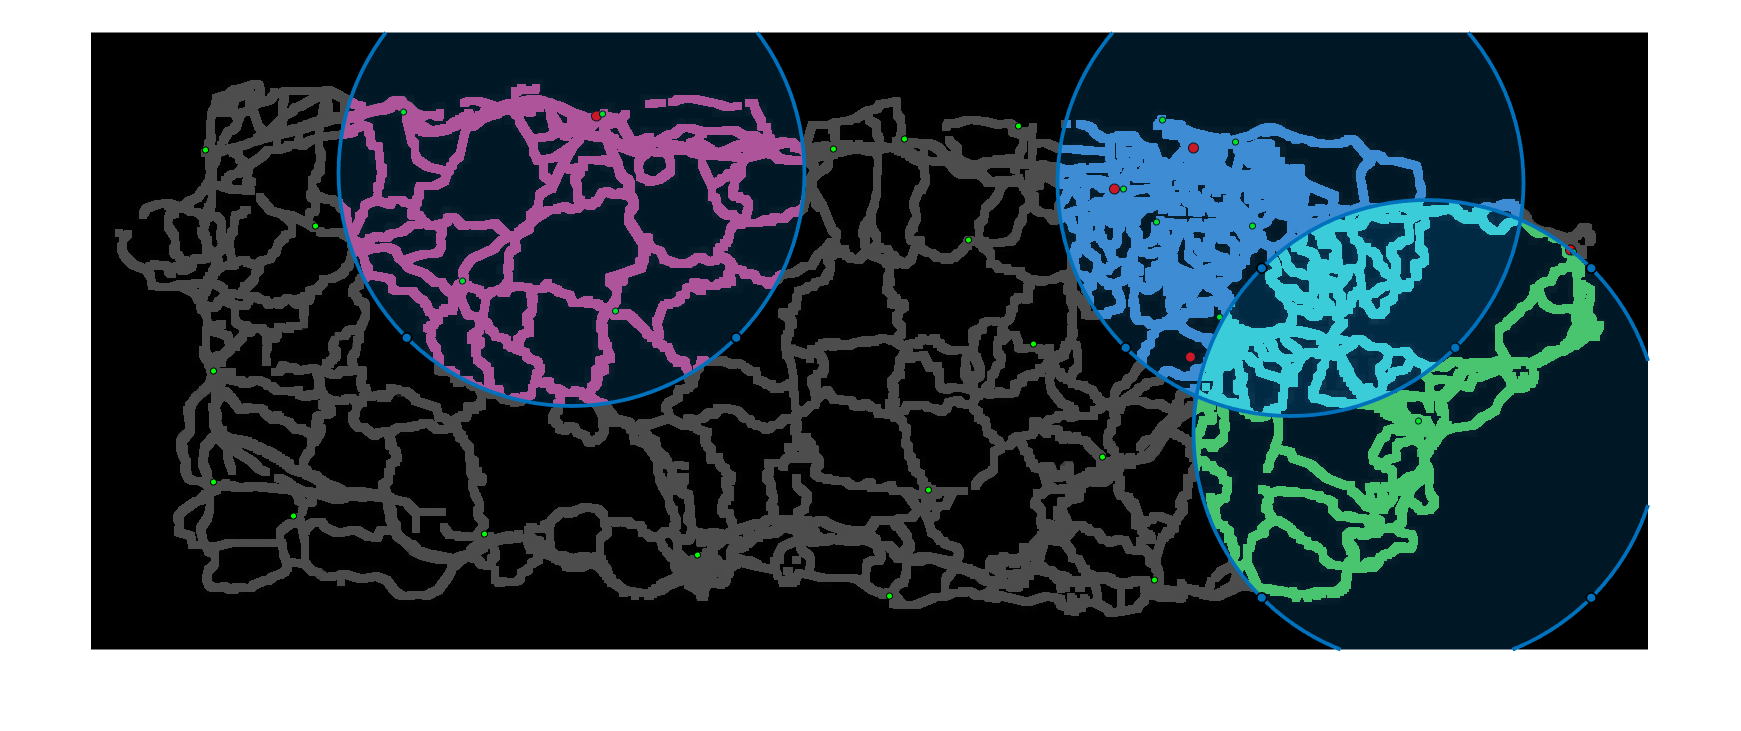
\includegraphics[scale=0.2]{2.png}
    \caption{ the City coordinates}
\end{figure}

\subsubsection{Extract All the Corners On The Map}
We use the RRT algorithm (because the RRT algorithm is more divergent than 
RRT-connect) for path planning from $[455, 1314]$ to $[338, 120]$ and $[452, 116]$.
Since the RRT algorithm will retrieve various possibilities in the form of 
numbers, it will traverse all possible nodes in the exploration.
\begin{figure}[h]
    \centering
    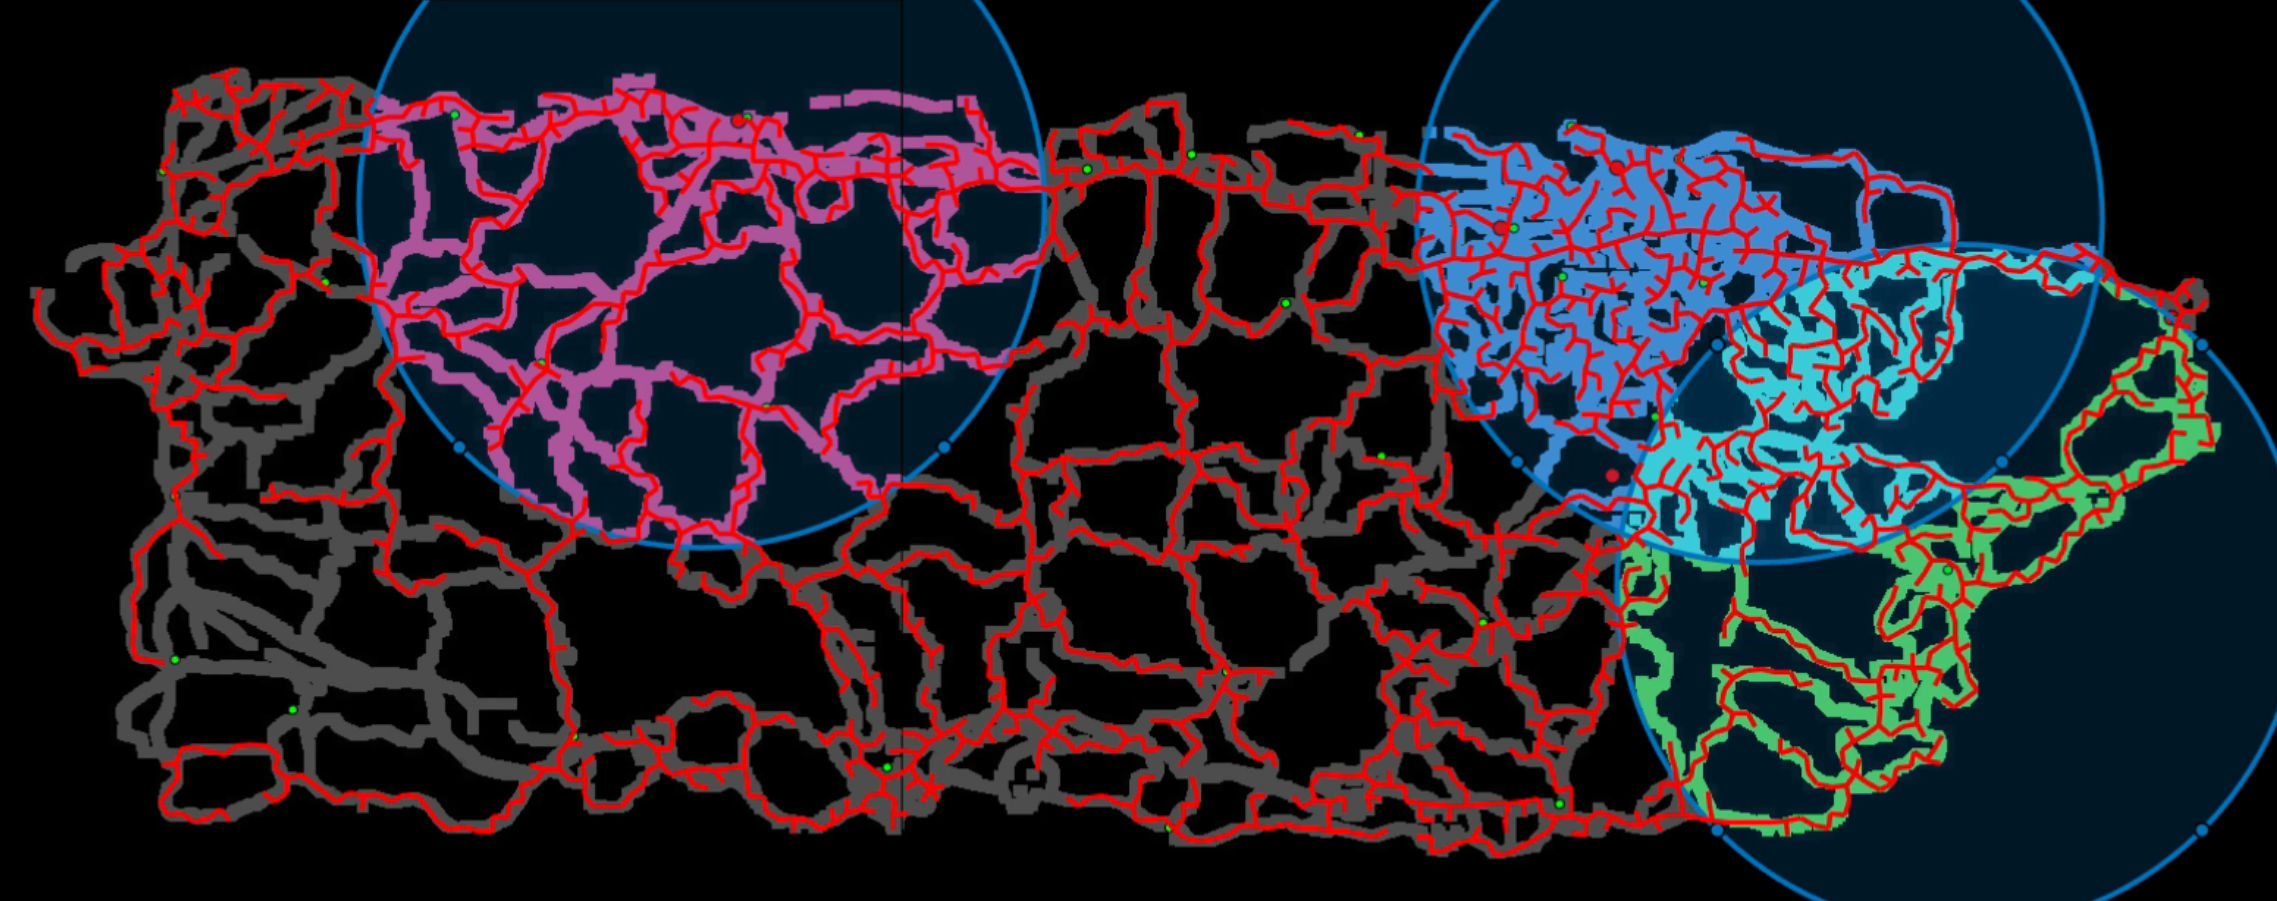
\includegraphics[scale=0.2]{all_nodes.png}
    \caption{The result of RRT-connect algorithm.}
\end{figure}

In this picture, we have drawn all possible road routes through matlab calculations, providing preparations for our next flight reconnaissance route selection.

\subsubsection{Path Planning And Trajectory Display}
From these city nodes that connect a route, we have selected several lines that mainly contact major cities to conduct drone reconnaissance activities
to provide accurate video information for our rescue.

The idea of RRT is to quickly expand a group of tree-like paths to explore most of the space 
and wait for opportunities to find a feasible paths. The "tree" was chosen because it explores space.


\begin{figure}[h]
    \centering
    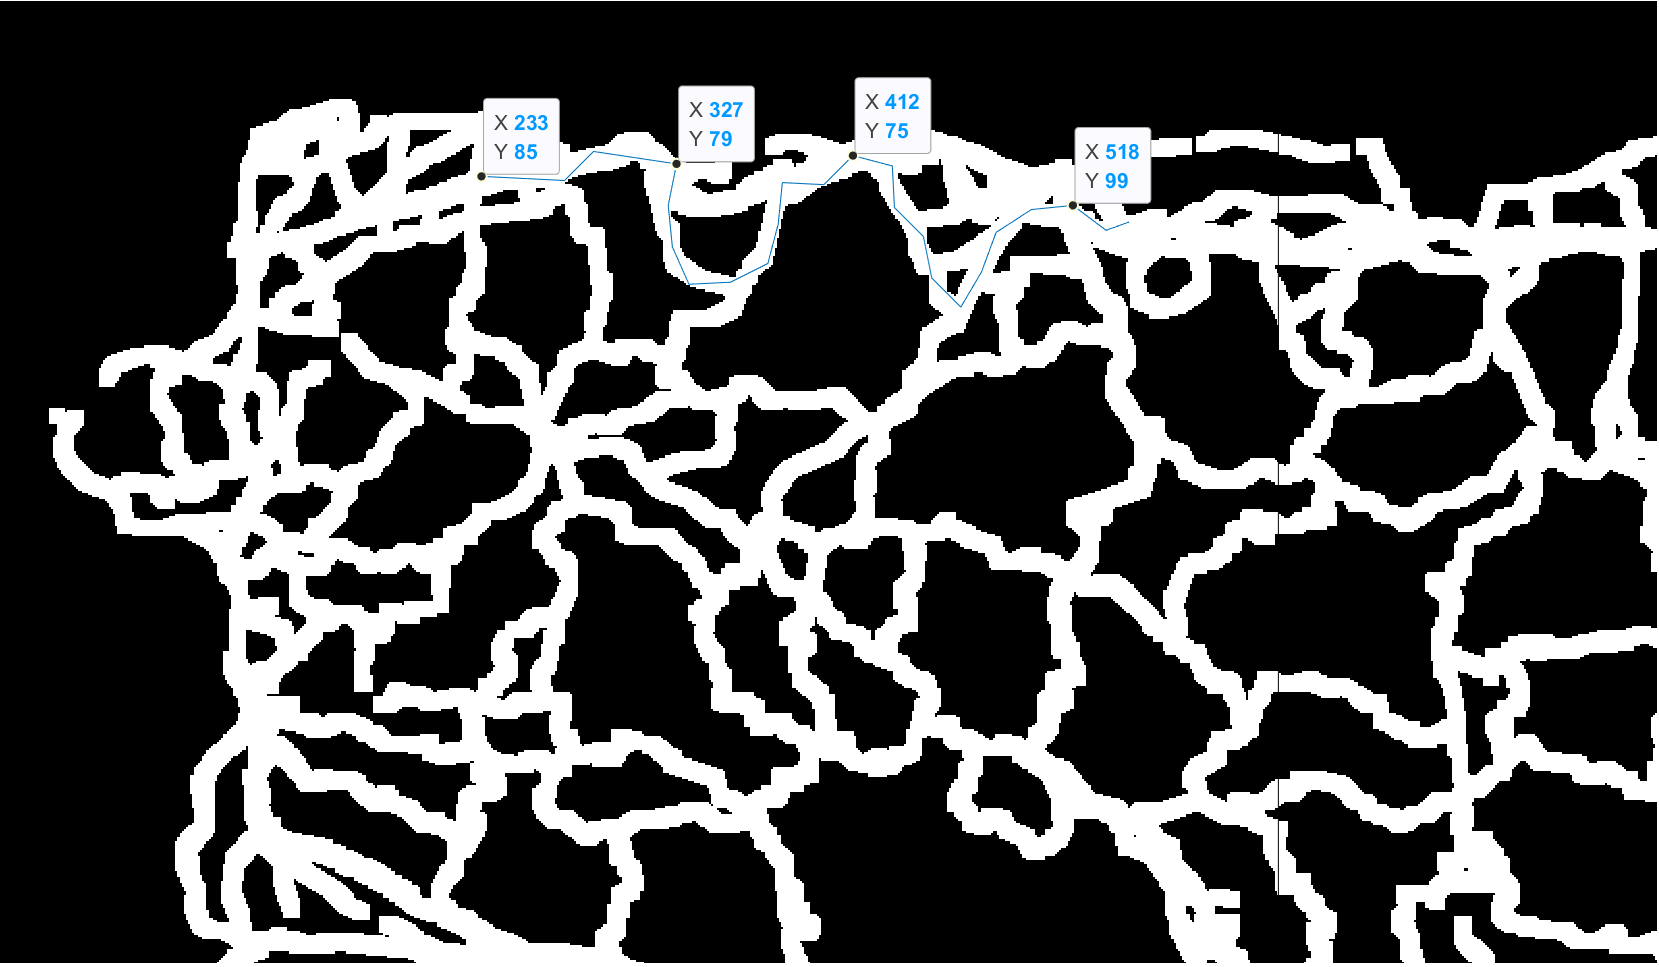
\includegraphics[scale=0.3]{sample_point_in_left_side_coastline.png}
    \caption{Sample points of the left side coastline obtained by RRT algorihm}
\end{figure}   


\begin{figure}[h]
        \centering
        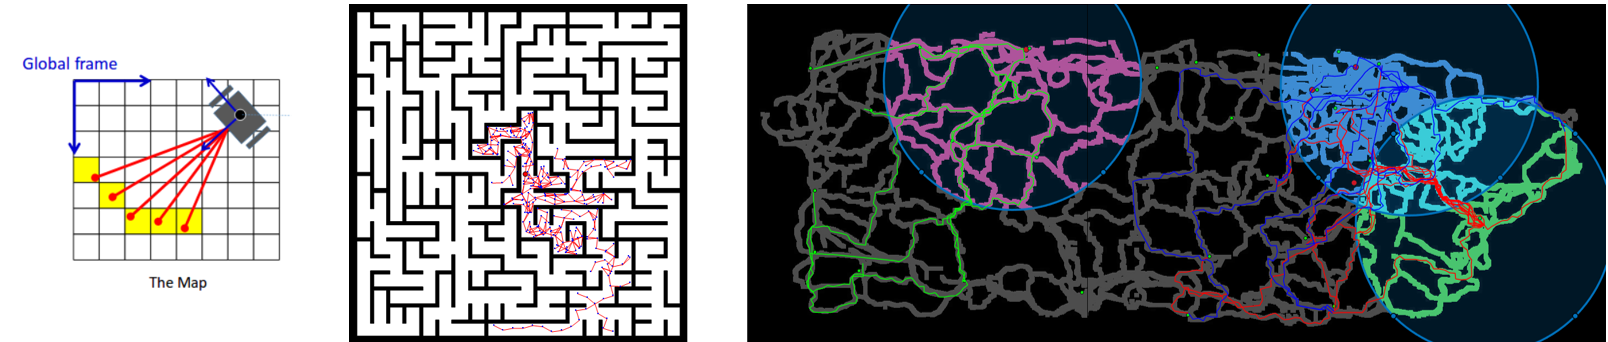
\includegraphics[scale=0.5]{RRT.png}
        \caption{The result of RRT-connect algorithm.}
    \end{figure}

    Among these selected routes, since some routes have a round-trip distance that greatly exceeds the maximum distance that the drone can fly and cannot return to the gathering point for charging, the drone we use is one-time.
    Our algorithm will be shown in a later appendix.
    

\section{Drone Flight Plan}
\subsection{Time Schedule}
% \begin{table}[]
%     \begin{tabular}{|c|c|c|l|}
%     \hline
%     \begin{tabular}[c]{@{}c@{}}Center\\ coordinates\\ (x,y)\end{tabular} & \begin{tabular}[c]{@{}c@{}}Area ratio of\\ reconnaissance\\ from the first\\ day to the\\ twentieth day\end{tabular} & \begin{tabular}[c]{@{}c@{}}Time required\\  in the \\ reconnaissance\\  circle\end{tabular} & \begin{tabular}[c]{@{}l@{}}The city that\\ scouted on\\ the 21st day\end{tabular}                                                        \\ \hline
%     (141,481)                                                            & 5\%-100\%                                                                                                            & 20 days                                                                                     & \begin{tabular}[c]{@{}l@{}}Aguadilla Pueblo\\ \&Hato Arriba \&\\  Mayagüez \&\\ Cabo Rojo\\ \& Ponce\\ \& Lajas \\ \& Yauco\end{tabular} \\ \hline
%     (151,1200)                                                           & 5\%-100\%                                                                                                            & 20 days                                                                                     & \begin{tabular}[c]{@{}l@{}}Manatí \& Vega Baja\\ \&Dorado \& Coamo\\ \&Santa Isabel\end{tabular}                                         \\ \hline
%     (401,1336)                                                           & 5\%-100\%                                                                                                            & 20 days                                                                                     & \begin{tabular}[c]{@{}l@{}}Salinas \& Palomas\\ \&Cayey \&\\ Guayama\end{tabular}                                                        \\ \hline
%     \end{tabular}
%     \end{table}

\section{Weakness}

    A weakness of RRT is that it is difficult to find a path in an environment with narrow passages. Because the narrow aisle area is small and the probability of being hit is low, the time required to find the path depends on luck.


\end{document}


